% \begin{figure}[htb]
%   \centering
%   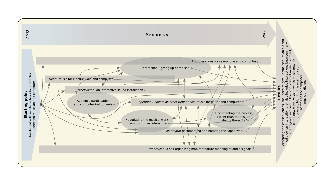
\includegraphics[width=\textwidth]{img/map8-noheader}
%   \caption{A timeline with the different sub-projects and themes with % their interrelations.}
%   \label{fig:main-map-ending}
% \end{figure}

%Accepting the consequences (the need to give up 'the Self') of an extended view on interaction that also includes interactions between many other agents involved in the production of musical content, led to new ways ways in which music may be produced, blurring the work concept as well as the composer-musician divide.

\begin{wrapfigure}{r}{0.24\linewidth}
\centering
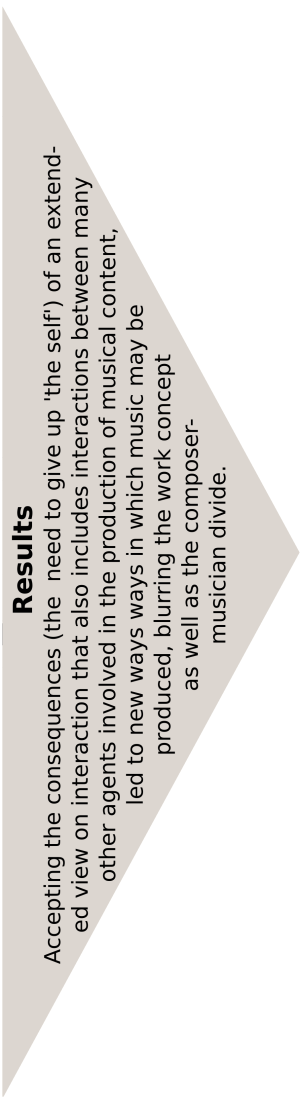
\includegraphics[width=0.95\linewidth]{img/map8-results.png}
\end{wrapfigure}
Throughout this project I have tried to understand what it means to play with, on, and through computers, alone and with others. At the outset I could not have imagined that the idea of \emph{resisting control} would be the pivotal concept. In fact, I was convinced that Interactive Music was about \emph{gaining} control over the computer as a first step towards a more dynamic \useGlosentry{glos:musician}{musician}-\index{interaction!computer}computer interaction. With hindsight, of course, I can see that the dissociation from \index{interaction!as control}interaction-as-control had always been there. Neither could I have anticipated that a return to a more radical improvisatory attitude towards \emph{all} aspects of my musical practice would be one of the outcomes. Common to both of these concepts, the giving up of control, and the improvisatory attitude (which are not necessarily symmetrical; an improvisatory attitude does not inevitably resist control methodologies) is the notion of giving up the \index{Self}Self. To me, the reciprocity of \index{interaction!social}social interaction assumes that those engaged in the interaction unleash some part of their Selves or else the communication in the interaction would simply bounce off the unchangeable, morphous egos. Interaction should lead to some kind of change, it should induce a \emph{difference} (that makes a difference) and only if the \index{Self}Self is prepared to accept difference will this be possible.

The extended view on \index{interaction!human-computer}\index{HCI}human-computer interaction that I have presented here, along with the blurred work concept and a developed (i.e. different from Eco's definition) concept of \useGlosentry{glos:work_in_movement}{work-in-movement}, led to the need to explore the significance of giving up the \index{Self}Self.  At the same time, however, the processes launched by this project would not have reached the work-in-motion or \index{interaction!as difference}\index{interaction-as-difference}interaction-as-difference had I not already started to let go of the Self. But what part of the \index{Self}Self is to be abandoned? Is any part of the \index{Self}Self at all retractable? The point here is not to show that by deserting some part of subjectivity, another, `truer', unconscious identity hidden below, deeper down, is revealed. It is a common mistake, also produced by psycho-analysis itself, to believe that the Freudian unconscious would be served well by being disclosed, made conscious: ``The unconscious is understood as a negative, it's the enemy.''\footcites[][57]{deleuze77}[See also][128-56]{bateson72} The \index{Self}Self is not first and foremost given up to discover something \emph{within}, but to become more resonant to that by which it is surrounded. Then the innermost part of the \index{Self}Self, conscious or unconscious, will also be affected. Jacques \citeauthor{attali85} writes that when ``music ceases to be catharsis; it no longer constructs differences. \emph{It is trapped in identity and will dissolve into noise}''.\footcite[45]{attali85} Similarly, I would like to propose that unless the \index{Self}Self allows for \index{interaction!as difference}\index{interaction-as-difference}interaction-as-difference, allows for the Other to play an active part in the interaction, the \index{Self}Self will cease to produce difference as well as cease to apprehend difference and will be trapped in its own identity.

The idea of the \index{Self}Self as soluble in artistic practice and music in particular is not new, nor is it original.\footnote{Although the field of art activity appears to me to have produced more egos than it has dissolved.} To philosopher Julius T. \citeauthor{fraser90}, the way music (and dance) embraces all levels of temporality it in some cases leads to the ``loss of individuality and establishes timeless belonging''.\footcite[410-1]{fraser90} Just as Brandon \citeauthor{labelle06}, with reference to Robin Maconie, talks about how ``sound and the self are wrapped up together'',\footcite[62]{labelle06} multimedia artist Frances Dyson similarly points to the intermingling of sound and identity: ``sound at the same time destroys the possibility of distinguishing between subject and environment, self and other, interior and exterior. Immersed in sound, the subject thus loses its self''. Furthermore, \citeauthor{labelle06}'s book \citetitle{labelle06} is an historical overview of concepts related to the loss of the \index{Self}Self in the context of sound art, music, and architecture, starting with John Cage and proceeding to the present day. In particular is the discussion in Part 3 of the book, relating to the voice is interesting in the present context and in an analysis of Marina Abramovic's performance \emph{Freeing the Voice} (1975), \citeauthor{labelle06} writes that she ``enacts the dynamic of speech as being, in one and the same instant, a process of losing and regaining oneself---that is, a form of catharsis''.\footcite[103]{labelle06} \citeauthor{labelle06} also discusses Alvin \citeauthor{lucier69}'s brilliant 1969 piece of sound art \citetitle{lucier69}, which is perhaps one of the more palpable examples of loss of the \index{Self}Self in sound. The score for the piece consists of a written instruction to sit down in a room with a microphone, two tape recorders, an amplifier and speakers. To play the piece is to read the specified text and record it onto one of the tape recorders and then play it back into the room while recording it onto the second tape recorder, after which the newly-recorded version is played back and recorded, etc. The effect is that eventually the spoken words begin to deteriorate and the resonances of the room take over. The \index{Self}Self, as constituted by the voice, is completely decomposed and immersed in the room.

\index{interaction!as control}Interaction-as-control and \index{interaction!as difference}\index{interaction-as-difference}interaction-as-difference are not opposites. They are complementary concepts in the large domain of \index{interaction!human-computer}\index{HCI}human-computer interaction. As noted above, at the beginning of the project I was expecting to have to develop my skills in order to build tools for better and more precise control of the computer in order to let go of the control agency and start thinking about more dynamic agencies. This is along the lines of the common, Western, ideal of learning and knowledge; develop a skill and master it. Perfect the skill and avoid mistakes. Although traditional conservatory training functions along the same lines, in much artistic practice, and in improvisation in particular, the mistake is a fundamental agent, a source of inspiration not to be avoided.\footcite[See][148-60]{evens05} But a mistake occurs only if I allow it to happen and will go unnoticed if I lack the skill or the insight to realise it has happened. The mistake depends on skill. It too is a difference that I will fail to detect if I am unable to understand what was mistaken. In other words, a certain amount of control is necessary in order to give up control. And the balance between `control' and `lose control', between \index{Self}Self and giving up of the \index{Self}Self, is a deceitful one. The story narrated by John \citeauthor{corbett94} in his book \citetitle{corbett94} of how drummer Milford Graves manages to stop his heart from beating at will prior to playing a solo concert is perhaps one of the more radical examples of \emph{controlling} the loss of the \index{Self}Self.\footnote{Graves's solo playing in general is an excellent example of how the most intimate and detailed level of physical control is dissolved in what I perceive as the most incredible freedom.} What could be a more radical way of losing the \index{Self}Self than to stop one's heart at will?\footcite[74]{corbett94} The computer, however, is a phenomenal losing-control and forgetting machine, in this context a less lethal one. As remarked in many places throughout this text it increases resistance and introduces dualities and alternate personalities in a way that forces one to constantly relocate or give up the \index{Self}Self. It is similar to how Ornette Coleman's playing of the trumpet and the violin introduces resistance, forces Coleman to give up part of the skill he acquired on the saxophone; similar to how Marcel Duchamp used mechanical drawing in order to ``avoid the old-fashioned form of drawing'', to forget with his hand\footcite[Duchamp quoted in][29]{tomkins65} and how Paul D. \citeauthor{miller08} (DJ Spooky) uses turntables to forget: ``it seemed that turntables were somehow imbued with the art of being memory permutation machines. They changed how I remembered sounds and always made me think of a different experience with each listening''.\footcite[45]{miller04} It is my aim to continue to learn the computer, learn its languages and its methods, in order to forget and thus allow for novel experiences. Control (by learning I gain control) as an instrument also to lose control (by forgetting).

To resist control, then, is as much a posture as it is a different kind of (implementation of) \index{interaction!human-computer}\index{HCI}human-computer interaction and in this sense it is related to improvisation. Again, risking triggering an ideological debate on composition versus improvisation (see \hyperref[sec:personal-background]{Section \ref*{sec:personal-background}}), I believe there is a relation between these two musical practices somewhat similar to the relation between \index{interaction!as control}\index{interaction-as-control}interaction-as-control and \index{interaction!as difference}\index{interaction-as-difference}interaction-as-difference. On the one hand stands the ostensible sense of control that the finalised musical score, sometimes homologous to \emph{the work}, offers its composer in its flat surface representation of ``musical formalism [\ldots] entirely divorced from any relationship to intuitive gestural experience''.\footcite[35]{wis96} On the other hand stands the likewise apparent \emph{freedom} of musical improvisation which in some cases and under certain conditions is anything but formalised.\footnote{In other cases it is as formalised as any compositional practice.} Composition, and the printed score, as a means to gain control over one's own music, to make it tangible, archivable and sustainable. Improvisation as a practice to create differences that loses meaning outside the context against which the difference is created. But, once more, \index{interaction!as difference}\index{interaction-as-difference}interaction-as-difference is also an attitude. An attitude that can be applied to the practice of composition which is seen in \emph{Drive} and 
\emph{Repetition Repeats all other Repetitions}, and an attitude that may be supported by the technologies and ideas that have been developed within the framework of \emph{libIntegra}. 

%\begin{wrapfigure}{r}{0.45\linewidth}
  \begin{minipage}[h]{\linewidth}
    \begin{flushright}
      \musicannot{Drive\\
        \emph{for Electric Viola Grande and computer}\\
        Composed \& premiered in 2002\\
        Commissioned by and dedicated to Henrik Frendin}
    \end{flushright}
  \end{minipage}
\end{wrapfigure}

%%% Local Variables: 
%%% mode: latex
%%% TeX-master: "../ImprovisationComputersInteraction"
%%% End: 

Although I was yet unaware of it, the change was already noticeable in the earliest artistic sub-project, \emph{Drive}. In the interaction between Frendin and me the significance of the roles of composer and performer had already begun to wear off, but the sub-project that induced the \emph{difference} that made me aware of my unresolved need for control was \emph{etherSound}. After the initial excitement of having set everything up and experienced the installation working, I had to face the fear that I could not, in fact, fully control the output. First of all because it would be impossible to be physically present at all times: the installation would be active for three weeks, ten hours a day; second because the participants would have their own will and their own ideas of when and how to contribute. Even though the idea for \emph{etherSound} had come up in collaboration with the curator Miya Yoshida, I had programmed it myself. In other words, similarly to how it is described in \hyperlink{sec:target:overview-1}{the Introduction}, I as a detached \index{Self}Self did the programming of \emph{etherSound} and created a situation that I as the situated \index{Self}Self and as composer felt deeply uncomfortable with. In the interaction with my \index{Self}Self, mediated through the computer, a difference was induced thanks to which I learned the importance of giving up some part of that same \index{Self}Self. 

%\begin{wrapfigure}{r}{0.45\linewidth}
  \begin{minipage}[h]{\linewidth}
    \begin{flushright}
      \musicannot{Repetition Repeats all other Repetitions\\
        \emph{for ten-stringed guitar and computer}\\
        Composed \& premiered in 2006\\
        Commissioned by and dedicated to Stefan \"{O}stersj\"{o}}
    \end{flushright}
  \end{minipage}
\end{wrapfigure}

%%% Local Variables: 
%%% mode: latex
%%% TeX-master: "../ImprovisationComputersInteraction"
%%% End: 

Within \emph{Repetition Repeats all other Repetitions} the intellectual understanding of the phenomena I had already experienced began to take shape. In the collaboration between Stefan \"{O}stersj\"{o} and Love Mangs these aspects of interaction and the \index{Self}Self were seen in a new light. The understanding of composition as a negotiation, regardless of what level of interaction the composing is part of, paved the way for a different understanding of the practice of composition. It was, however, in the radical way that we gave up the notion of \emph{the work}, and even the \emph{open work} and established a re-interpretation of Eco's \emph{work-in-movement} that the full consequences of my altered composer role became evident. The \useGlosentry{glos:work_in_movement}{work-in-movement} is focused on the process rather than the result, in itself not a novel idea at all. In the context of computers and interaction and in combination with the idea of the augmented score, however, the focus on the process allowed an altered view on musical interpretation as well as composition: the score as a growing container of musical experience (rather than a detailed instruction to be rigorously followed), all of which is open-sourced to allow for any kind of transformation but with the request to let the interactive narrative, the collaboration, guide the additions, alterations and removals of material from the score.

%\begin{wrapfigure}{r}{0.4\linewidth}
  \begin{minipage}[h]{\linewidth}
    \begin{flushright}
      \musicannot{IntegraBrowser\\
        \emph{Offline browser for the Integra XML\\documentation format.}}
    \end{flushright}
  \end{minipage}
\end{wrapfigure}

%%% Local Variables: 
%%% mode: latex
%%% TeX-master: "../ImprovisationComputersInteraction"
%%% End: 

\emph{libIntegra} is the glue that potentially can make interaction simpler between environments for live \index{electro-acoustic music}electro-acoustic music. Not only is the augmented score enabled by aspects of libIntegra, but the fact that the \useGlosentry{glos:dsp}{DSP} modules, environments and stand-alone programs which may be described, shared and communicated in a uniform and abstract way are integral aspects of \emph{libIntegra} and furthers the idea of the \useGlosentry{glos:work_in_movement}{work-in-movement}. The core definitions of the protocol have been defined as openly as possible in order to allow for a widespread and distributed community to contribute to its expansion. 

These four mapped projects, \emph{Drive}, \emph{etherSound}, \emph{Repetition\ldots} and \emph{libIntegra} are framed by the improvisations and \emph{timbreMap} (see Figure \ref{fig:main-map}; by the most elusive and abstract (improvisation) and the most formal and concrete (programming). Now both of these are also in themselves representatives of the abstract-concrete opposition: improvising \emph{with} computer and a computer program that interacts with \emph{sound}. Improvisation, computer, sound. Integrated by interaction. Improvisation communicated to the computer, mediated by sound. The computer communicating with the improviser, mediated by sound. Sound as the interface. Since timbre (the quality of the sound/interface), can only be described in terms of \emph{difference} from other timbres surrounding it (leaving any theory of a general sound morphology aside),\footnote{Timbre, according to OED, is ``The character or quality of a musical or vocal sound (distinct from its pitch and intensity) [\ldots] distinguishing it from sounds proceeding from other sources'' \cite{timbre-oed}} the sound/interface is in itself a kind of difference: \index{interaction!as difference}\index{interaction-as-difference}interaction-as-difference. Furthermore, the map is a good visual representation of the function of time in the interactive system; it can even be seen as a graphic representation of the interaction between the different sub-projects. Time has been the topic in several sections, and the difference between parallel motion systems, systems that have some notion of time, however limited, and trigger-event systems, pure stimuli-response systems with no recollection of prior events, was discussed in \hyperref[sec:drive-2003]{Section \ref*{sec:drive-2003}}. This project is and has been a parallel motion system. The different sub-projects have informed each other but they have maintained their forward motion independently of each other in a way similar to how \emph{Drive} is portrayed in \hyperref[fig:parllel]{Figure \ref*{fig:parllel}}.

The six trajectories that took me from the starting-point to here, to the next beginning, have helped me better understand the concepts of interaction, openness, \index{Self}Self and control. But as containers they also hold some of the knowledge within them, and, owing to the intended open form and the fact that each of these projects can take off on its own, independent of my involvement and consent, whatever knowledge is encoded in them will then continue to develop. I propose an open-source music that is not only the \emph{grab-and-play} of P2P\footnote{Peer-to-peer networks are used widely for file sharing purposes.} and Bit Torrents but more of a distribution of construction kits. Build your own music. \citeauthor{corbett94}, leaning on Jacques Attali,\footcite[See][]{attali85} writes how ``improvising musicians create a genuine Deleuzian assemblage, a musical machine of desire---not binary, nor unitary, but multiple''.\footcite[76]{corbett94} Why should the musical assemblage be limited to improvising musicians? I am aiming at an even more decentralised assemblage (although it, too, will have to deal with limitations, for it is dependent on computers and networks). Central to the idea of the musical open-source is the reciprocity; what is taken is altered and returned and thus added to all other contributions. Each such bundle of musical practice that holds within it multiple relations and multiple kinds of interaction is a veritable work-in-movement, truly moving around in a way I am sure Eco did not anticipate.
\newpage
\thispagestyle{empty}

%But if it is not possible to control technology and it is not possible to give up technology, then our only choice is to stop \emph{trying} to control it and accept it as a, this time truly epistemological Other.

%%% Local Variables: 
%%% mode: latex
%%% TeX-master: "../ImprovisationComputersInteraction"
%%% End: 
